\begin{subfigure}[b]{0.30\textwidth}
    \centering
    \resizebox{\linewidth}{!}{
        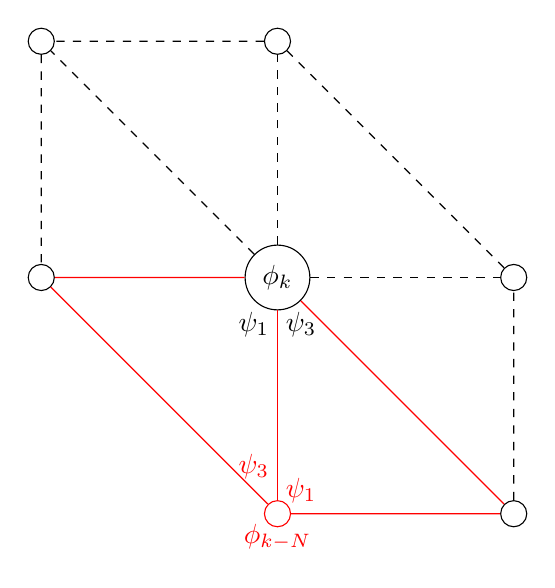
\begin{tikzpicture}[scale=3]
            % Place the center node
            \node[circle,draw=black] (k) at (0,0) {$\phi_k$};
            \node (p1) at (0.1, -0.2) {$\psi_3$};
            \node (p2) at (-0.1, -0.2) {$\psi_1$};
            \node (p2) at (-0.1, -0.8) {\color{red}$\psi_3$};
            \node (p1) at (0.1, -0.9) {\color{red}$\psi_1$};

            % Place the other nodes
            \node[circle,draw=black] (x0) at (-1,0) {};
            \node[circle,draw=red] (x1) at (0,-1) {};
            \node (k1) at (0, -1.1) {\color{red}$\phi_{k-N}$};
            \node[circle,draw=black] (x2) at (-1,1) {};
            \node[circle,draw=black] (x3) at (1,-1) {};
            \node[circle,draw=black] (x4) at (1,0) {};
            \node[circle,draw=black] (x5) at (0,1) {};

            % The lines!
            \draw[red] (k) -- (x0) -- (x1) -- (x3) -- (k);
            \draw[red] (k) -- (x1);
            \draw[dashed] (x3) -- (x4) -- (x5) -- (x2) -- (x0);
            \draw[dashed] (k) -- (x4);
            \draw[dashed] (k) -- (x5);
            \draw[dashed] (k) -- (x2);
        \end{tikzpicture}}
\end{subfigure}
\begin{subfigure}[b]{0.30\textwidth}
    \centering
    \resizebox{\linewidth}{!}{
        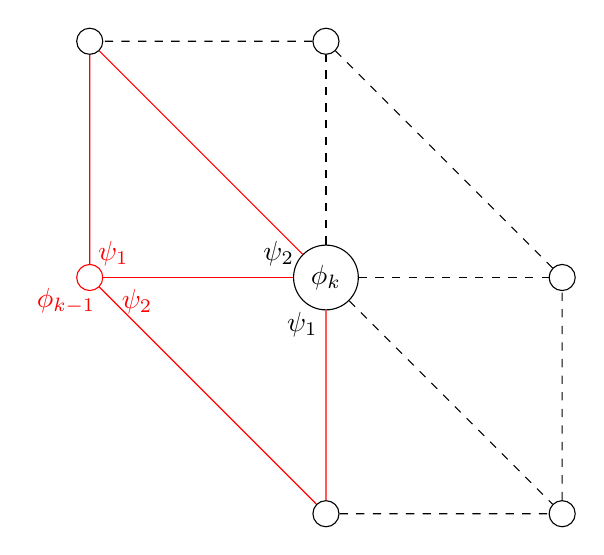
\begin{tikzpicture}[scale=3]
            % Place the center node
            \node[circle,draw=black] (k) at (0,0) {$\phi_k$};
            \node (p1) at (-0.2, 0.1) {$\psi_2$};
            \node (p2) at (-0.1, -0.2) {$\psi_1$};
            \node (p2) at (-0.8, -0.1) {\color{red}$\psi_2$};
            \node (p1) at (-0.9, 0.1) {\color{red}$\psi_1$};

            % Place the other nodes
            \node[circle,draw=red] (x0) at (-1,0) {};
            \node (k1) at (-1.1, -0.1) {\color{red}$\phi_{k-1}$};
            \node[circle,draw=black] (x1) at (0,-1) {};
            \node[circle,draw=black] (x2) at (-1,1) {};
            \node[circle,draw=black] (x3) at (1,-1) {};
            \node[circle,draw=black] (x4) at (1,0) {};
            \node[circle,draw=black] (x5) at (0,1) {};

            % The lines!
            \draw[red] (k) -- (x1) -- (x0) -- (x2) -- (k);
            \draw[red] (k) -- (x0);
            \draw[dashed] (x1) -- (x3) -- (x4) -- (x5) -- (x2);
            \draw[dashed] (k) -- (x5);
            \draw[dashed] (k) -- (x3);
            \draw[dashed] (k) -- (x4);
        \end{tikzpicture}}
\end{subfigure}
\begin{subfigure}[b]{0.30\textwidth}
    \centering
    \resizebox{\linewidth}{!}{
        \begin{tikzpicture}[scale=3]
            % Place the center node
            \node[circle,draw=black] (k) at (0,0) {$\phi_k$};
            \node (p1) at (-0.2, 0.1) {$\psi_2$};
            \node (p2) at (-0.1, 0.25) {$\psi_3$};
            \node (p2) at (-0.8, 0.9) {\color{red}$\psi_2$};
            \node (p1) at (-0.9, 0.8) {\color{red}$\psi_3$};

            % Place the other nodes
            \node[circle,draw=black] (x0) at (-1,0) {};
            \node[circle,draw=black] (x1) at (0,-1) {};
            \node[circle,draw=red] (x2) at (-1,1) {};
            \node (k1) at (-1, 1.15) {\color{red}$\phi_{(k-1) + N}$};
            \node[circle,draw=black] (x3) at (1,-1) {};
            \node[circle,draw=black] (x4) at (1,0) {};
            \node[circle,draw=black] (x5) at (0,1) {};

            % The lines!
            \draw[red] (k) -- (x5) -- (x2) -- (x0) -- (k);
            \draw[red] (k) -- (x2);
            \draw[dashed] (x0) -- (x1) -- (x3) -- (x4) -- (x5);
            \draw[dashed] (k) -- (x1);
            \draw[dashed] (k) -- (x3);
            \draw[dashed] (k) -- (x4);
        \end{tikzpicture}}
\end{subfigure}
\begin{subfigure}[b]{0.30\textwidth}
    \centering
    \resizebox{\linewidth}{!}{
        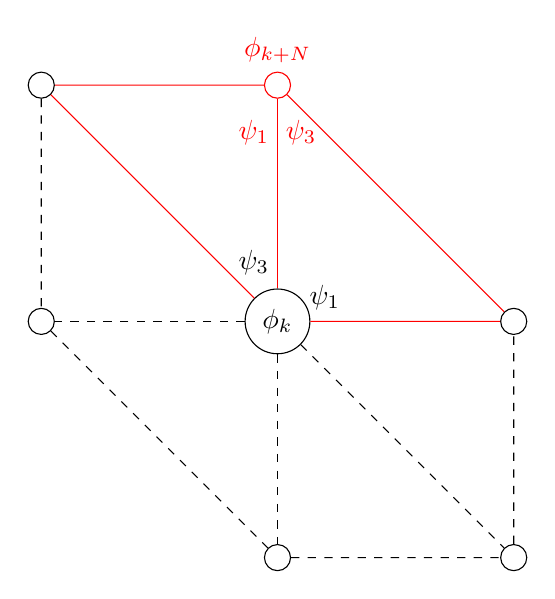
\begin{tikzpicture}[scale=3]
            % Place the center node
            \node[circle,draw=black] (k) at (0,0) {$\phi_k$};
            \node (p1) at (0.2, 0.1) {$\psi_1$};
            \node (p2) at (-0.1, 0.25) {$\psi_3$};
            \node (p2) at (0.1, 0.8) {\color{red}$\psi_3$};
            \node (p1) at (-0.1, 0.8) {\color{red}$\psi_1$};

            % Place the other nodes
            \node[circle,draw=black] (x0) at (-1,0) {};
            \node[circle,draw=black] (x1) at (0,-1) {};
            \node[circle,draw=black] (x2) at (-1,1) {};
            \node[circle,draw=black] (x3) at (1,-1) {};
            \node[circle,draw=black] (x4) at (1,0) {};
            \node[circle,draw=red] (x5) at (0,1) {};
            \node (k1) at (0, 1.15) {\color{red}$\phi_{k + N}$};

            % The lines!
            \draw[red] (k) -- (x4) -- (x5) -- (x2) -- (k);
            \draw[red] (k) -- (x5);
            \draw[dashed] (x2) -- (x0) -- (x1) -- (x3) -- (x4);
            \draw[dashed] (k) -- (x0);
            \draw[dashed] (k) -- (x1);
            \draw[dashed] (k) -- (x3);
        \end{tikzpicture}}
\end{subfigure}
\begin{subfigure}[b]{0.30\textwidth}
    \centering
    \resizebox{\linewidth}{!}{
        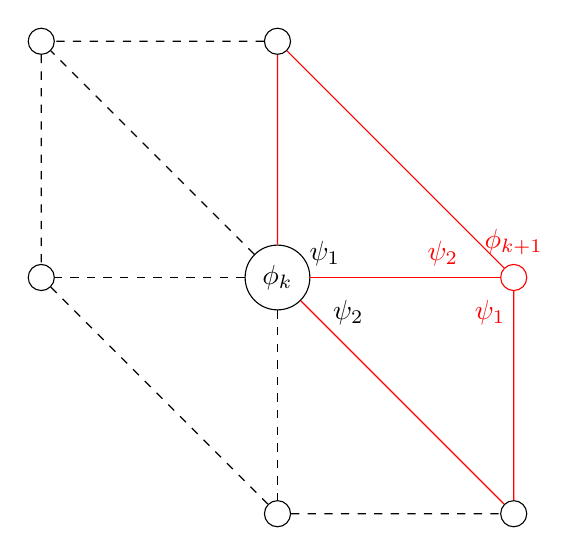
\begin{tikzpicture}[scale=3]
            % Place the center node
            \node[circle,draw=black] (k) at (0,0) {$\phi_k$};
            \node (p1) at (0.2, 0.1) {$\psi_1$};
            \node (p2) at (0.3, -0.15) {$\psi_2$};
            \node (p2) at (0.7, 0.1) {\color{red}$\psi_2$};
            \node (p1) at (0.9, -0.15) {\color{red}$\psi_1$};

            % Place the other nodes
            \node[circle,draw=black] (x0) at (-1,0) {};
            \node[circle,draw=black] (x1) at (0,-1) {};
            \node[circle,draw=black] (x2) at (-1,1) {};
            \node[circle,draw=black] (x3) at (1,-1) {};
            \node[circle,draw=red] (x4) at (1,0) {};
            \node (k1) at (1, 0.15) {\color{red}$\phi_{k+1}$};
            \node[circle,draw=black] (x5) at (0,1) {};

            % The lines!
            \draw[dashed] (x5) -- (x2) -- (x0) -- (x1) -- (x3);
            \draw[dashed] (k) -- (x2);
            \draw[dashed] (k) -- (x0);
            \draw[dashed] (k) -- (x1);
            \draw[red] (k) -- (x3) -- (x4) -- (x5) -- (k);
            \draw[red] (k) -- (x4);
        \end{tikzpicture}}
\end{subfigure}
\begin{subfigure}[b]{0.30\textwidth}
    \centering
    \resizebox{\linewidth}{!}{
        \begin{tikzpicture}[scale=3]
            % Place the center node
            \node[circle,draw=black] (k) at (0,0) {$\phi_k$};
            \node (p3) at (0.1, -0.3) {$\psi_3$};
            \node (p2) at (0.4, -0.15) {$\psi_2$};
            \node (p2) at (0.6, -0.9) {\color{red}$\psi_2$};
            \node (p3) at (0.9, -0.7) {\color{red}$\psi_3$};

            % Place the other nodes
            \node[circle,draw=black] (x0) at (-1,0) {};
            \node[circle,draw=black] (x1) at (0,-1) {};
            \node[circle,draw=black] (x2) at (-1,1) {};
            \node[circle,draw=red] (x3) at (1,-1) {};
            \node (k1) at (1, -1.1) {\color{red}$\phi_{(k + 1) - N}$};
            \node[circle,draw=black] (x4) at (1,0) {};
            \node[circle,draw=black] (x5) at (0,1) {};

            % The lines!
            \draw[dashed] (x4) -- (x5) -- (x2) -- (x0) -- (x1);
            \draw[dashed] (k) -- (x5);
            \draw[dashed] (k) -- (x2);
            \draw[dashed] (k) -- (x0);
            \draw[red] (k) -- (x1) -- (x3) -- (x4) -- (k);
            \draw[red] (k) -- (x3);
        \end{tikzpicture}}
\end{subfigure}
\begin{subfigure}[b]{0.30\textwidth}
    \centering
    \resizebox{\linewidth}{!}{
        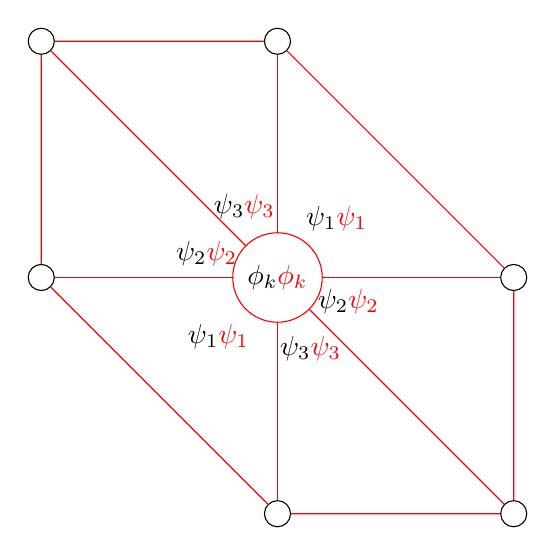
\begin{tikzpicture}[scale=3]
            % Place the center node
            \node[circle,draw=red] (k) at (0,0) {$\phi_k
                                                  \color{red}\phi_k$};
            \node (p1) at (0.14, -0.3){$\psi_3\color{red}\psi_3$};
            \node (p4) at (-0.14, 0.3) {$\psi_3\color{red}\psi_3$};
            \node (p2) at (-0.25, -0.25) {$\psi_1\color{red}\psi_1$};
            \node (p3) at (0.25, 0.25) {$\psi_1\color{red}\psi_1$};
            \node (p5) at (0.3, -0.1) {$\psi_2\color{red}\psi_2$};
            \node (p6) at (-0.3, 0.1) {$\psi_2\color{red}\psi_2$};

            % Place the other nodes
            \node[circle,draw=black] (x0) at (-1,0) {};
            \node[circle,draw=black] (x1) at (0,-1) {};
            \node[circle,draw=black] (x2) at (-1,1) {};
            \node[circle,draw=black] (x3) at (1,-1) {};
            \node[circle,draw=black] (x4) at (1,0) {};
            \node[circle,draw=black] (x5) at (0,1) {};

            % The lines!
            \draw[red] (x0) -- (x1) -- (x3) -- (x4) -- (x5) -- (x2) -- (x0);
            \draw[red] (k) -- (x0);
            \draw[red] (k) -- (x1);
            \draw[red] (k) -- (x2);
            \draw[red] (k) -- (x3);
            \draw[red] (k) -- (x4);
            \draw[red] (k) -- (x5);
        \end{tikzpicture}}
\end{subfigure}
